\documentclass[12pt]{scrreprt}
\usepackage{graphicx}
\usepackage{geometry}
\geometry{
 a4paper,
 left=20mm,
 right=20mm,
 top=25mm,
 headheight=20mm,
 headsep=0mm,
 bottom=30mm,
}
\usepackage[T1]{fontenc}				% Trennung von Umlauten.
\usepackage[ngerman]{babel}	
\usepackage[utf8]{inputenc}
\usepackage[headsepline]{scrlayer-scrpage}
\ModifyLayer[addvoffset=-10pt]{scrheadings.head.below.line}
\usepackage{blindtext}
\usepackage[font=small,labelformat=empty,justification=centering]{caption}
\setlength{\parindent}{0em}

\usepackage[version=4]{mhchem}

%Autordaten
\newcommand{\datum}{02.07.2020}
\newcommand{\autorinfo}{\textbf{Wechler, Tim-Jonas} (1137877)}


\ihead{\textbf{WT 1} \datum}
\chead{\autorinfo}
\ohead{\vspace{10pt}
\includegraphics[width=4cm]{logo_simple}}
 
\begin{document}

Dieses Lerntagebuch ist nich wie bisher auf Basis eines Videos enstanden, sondern aus dem Skript in Eigenarbeit erstellt worden.\\
Die Kapitel die dieses mal behandelt wurden sind Ungleichgewichts-Gefüge und Stahlherstellung.\medskip

Im Kapitel \textbf{Ungleichgewichts-Gefüge} wurde uns näher gebracht das bei unterschiedlichen Abkühlgeschwindigkeiten unterschiedliche Phasenumwandlungen statt finden können. Im Kapitel ist man von der Phase Austenits ausgegangen. Erhöht man die Abkühlgeschwindigekeit bewirkt dies eine höhere Keimdichte und die ausbildung von Perlit.
Durch die Abkühlung wird die ausbildung bon rundlichen Gefügen unterdrückt worduch die Gefüge eine längliche oder falche From einnehmen. \smallskip

Die Phasenumwandlung ist wie schon erwähnt von der Zeit und Temperatur abhängig. Die Abkühlgeschwindigekeiten  unterteilt man in vier Stufen ein.\\
Die erste Stufe ist mit einem Kohlenstoffanteil von \(c = 0,8\%\) und einer moderaten  Abkühlgeschwindigekeit in der Lage alles in Perlit um zu wandeln. Mit steigender Geschwindigkeit wird der Gefügeabstand kleiner. 
Die nächste Stufe besteht aus feinem Perlit und ist nur unter einem Elektronenmikroskop zu erkennen. Die erste Stufe und diese Stufe werden auch alsi PerlitStufe bezeichnet.
Zwischenstufe, ist der Name der nächsten Stufe. In dieser Stufe können die Eisen-Atome nicht mehr bewegen, dahingegen aber die Kohlenstoff-Atome. Im Vergleich zur Perlitbildung ist dieser Prozess ausgehend von der Bildung Ferritkeimen und im anschluss die Karbidausscheidung. Das Gefüge, was sich hier ausbildet, weißt eine hohe Festigkeit und Zähigkit nach.
Die letzte Stufe wird Martensitstufe genannt. Hier ist die Unterkühlung so das auch der Kohlenstoff sich nicht mehr bewegt. Die starke Unterkühlung wirkt eine starke Reaktionskraft, die trotz der starken Hinderung der Kohlenstoffübersättigung die Umwandlung ermöglicht.\medskip

Dies läst sich alles in \textbf{Zeit-Temperatur-Umwandlungs-Diagramme} darstellen. Ich habe zu eben diesem im Internet etwas nach geschaut und auf der Seite \\
https://hps.hs-regensburg.de/heh39273/aufsaetze/ztu.pdf eine allgemeine Erklärung gefunden. Ein solches Diagramm wird die Abkühlgeschwindigekeit einer Legierung dargestellt. Der charakteristische C-Förmige Verlauf entsteht durch die Überlagerung der Beweglichkeit und des Umwandlungsverhaltens. Man unterscheidet hier zwei Typen von Diagramme, das isothermische und kontinuierliche Zeit-Temperatur-Umwandlungs-Diagramm. 
Das \textbf{isotherme Umwandlungsdiagramm} beschreibt die Umwandlung bei gleichbleibender Temperatur. Dieses Diagramm mit parallel zur Zeit-Achse gelesen werden. 
Das \textbf{kontinuierliche Umwandlungsdiagramm}  enthalten nicht nur die Phasenumwandlung sondern auch die Abkühlkurven. An den Schnittpunkten ist der prozentuale Anteil der Phase ab zu lesen. \medskip

Im Kapitel \textbf{Stahlherstellung} konnte man über den Hochofenprozess lesen. Eisen findet man in der Natur nur als Oxid oder Karbonat. Die Erze werden in den Hochofen gegeben und durch Reduktion der Oxide trennt man diese von dem Eisen. Mit der Aufnahme von Kohlenstoff sinkt die Schmelztemperatur von Eisen auf 1200 °C. Am Ende des Prozess erhält man Roheisen was technisch unbrauchbar ist. 
Dieses Roheisen muss im Anschluss von weiteren Unreinheiten beseitigt werden, was zur folge hat das der Kohlenstoffanteil mit sinkt. Um diesen wieder zu erhöhen wird das Eisen im Sauerstoff Blasverfahren oder im Elektrostahlverfahren nachbehandelt.  
Hat das Eisen seine gewünschte Eigenschaften und Mischungsverhältnise so wird es entweder gegoßen oder wie auf der nächsten Seite zu sehen zu einem theoretisch endlosen Stück Stahl gebracht, was man auch Stranggießen nennt.
Beim Stranggießenwird der Stahl zwischen zwei Kokillen eingeführt die sich permanent Bewegung um ein Anhaften an den Stahl zu verhindern. Sobald der Stahl die Kokillen verlässt hat er schon genug Festigkeit erlangt damit die Bramme über Rollen weiter transportiert werden kann. \medskip

Zum Abschluss muss ich sagen, da man dieses mal kein Video hatte was einen auf das vermeintlich Wichtige hinweist, sondern man musste sich selbst überlegen welchen Stellenwert ein jeder Abschnitt im Skript hatte. 


\begin{figure}[h]
	\centering
	% \textwidth bezieht sich nun auf die Minipage
	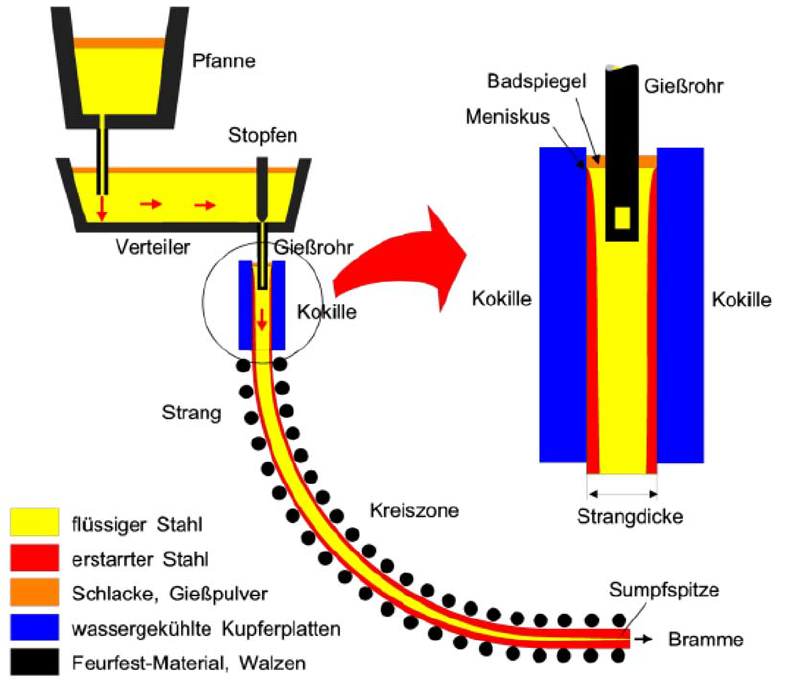
\includegraphics[width=0.7\textwidth]{stahl.png}
	\caption{Prinzip des Stranggießen\\(Quelle: Vorlesungsfolien WT1 Dr.\,E.Geberth)}
% \caption{noch eine Caption}
\end{figure}

\end{document}

